\section{Results}
\label{sec:results}

We organize results around the binary ambiguity effect (C1) and the type partial ordering (C2), both supported by our data, followed by the layer grouping (C3, inconclusive) and the model$\times$type interaction (C4, exploratory and driven by a single type).

\subsection{Binary Ambiguity Effect (C1)}

\begin{figure}[t]
\centering
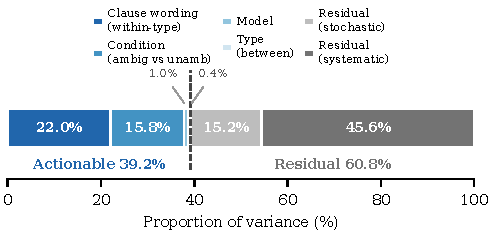
\includegraphics[width=\columnwidth]{figures/fig_variance_decomposition.pdf}
\caption{Variance decomposition of violation rates (temperature $= 0$). Clause identity: 22.4\% (0.4\% between types); condition: 15.8\%; model: 1.0\%; residual: 60.8\%. Clause wording---not type membership---is the primary risk factor among measured predictors.}
\label{fig:variance_decomposition}
\end{figure}

\begin{figure}[t]
\centering
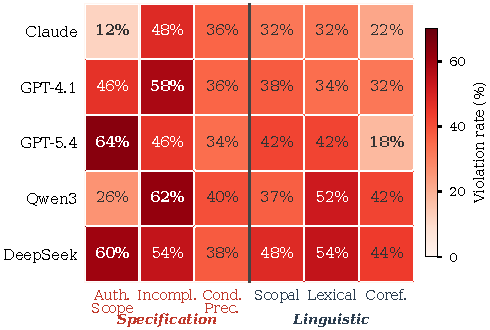
\includegraphics[width=\columnwidth]{figures/fig3_heatmap.pdf}
\caption{Violation rates (\%) by model and type under ambiguous conditions. Authorization scope shows the widest cross-model spread, reflecting differential safety training; incompleteness remains uniformly high (46--62\%) across all models.}
\label{fig:heatmap}
\end{figure}

Ambiguous policy clauses reliably increase safety violations across all models and ambiguity types. The overall effect is 34.0\,pp (41.0\% vs.\ 6.9\%; McNemar OR $= 15.1$, 95\% CI $[10.78, 21.17]$, $p < 10^{-105}$, based on $n = 580$ discordant pairs). The stratified Mantel--Haenszel OR is $9.57$ $[7.63, 12.01]$ (Appendix~\ref{app:mantel_haenszel}). All six types individually produce significant increases (all $p < 10^{-5}$) across both retail ($+$30.6\,pp) and airline ($+$37.7\,pp) domains (Appendix~\ref{app:cross_domain}), and all five models show large effects ($+25.7$ to $+39.0$\,pp, all $p < 10^{-17}$). Perturbation controls confirm specificity to semantic ambiguity (\S\ref{sec:method}). Figure~\ref{fig:variance_decomposition} decomposes violation-rate variance\footnote{Type III sum of squares (SS); logistic regression (Appendix~\ref{app:regression}) confirms concordant results (Tjur's $R^2 = 0.175$; \citealp{tjur_2009}).}: clause identity explains 22.4\% (0.4\% between types, 22.0\% within), condition 15.8\%, model 1.0\%, and residual 60.8\% ($\sim$15\% stochastic, $\sim$46\% systematic; Appendix~\ref{app:residual}). No single clause drives any type-level effect (Appendix~\ref{app:clause_variance}), and surface features are weak clause-level predictors (Appendix~\ref{app:clause_predictors}). Excluding incompleteness, which is subject to an information-addition confound (Appendix~\ref{app:confound}), the effect is $+$31.0\,pp (95\% CI $[27.9, 34.1]$; Appendix~\ref{app:sans_incompleteness}). The confound-minimized coreferential type still produces $+$18.7\,pp with only $\sim$7.8 words of token difference, isolating the ambiguity-only contribution. Authorization scope exhibits larger token differences ($\Delta = 36.1$ words; Appendix~\ref{app:clause_length}) without the information-addition confound. A logistic regression controlling for token-count differences confirms the effect persists at $\Delta_{\text{token}} = 0$ ($+$20.5\,pp, 95\% CI $[14.2, 26.8]$; Appendix~\ref{app:token_sensitivity}).

Convergent evidence from two additional models confirms the effect across seven models ($\Delta = +20.0$ to $+33.6$\,pp; Appendix~\ref{app:model_expansion}); cross-benchmark evaluation on SOPBench~\citep{li_sopbench_2025} shows directional consistency ($+12.7$\,pp unweighted mean; Appendix~\ref{app:sopbench}). Figure~\ref{fig:cross_benchmark} summarizes generalization across benchmarks. The taxonomy predicts failure mechanisms more strongly than violation rate (normalized mutual information, NMI $= 0.23$ vs.\ $0.01$; $V = 0.45$ vs.\ $0.14$ on tables of different dimensionality; Appendix~\ref{app:type_mechanism}), making type-level analysis (C2--C4) informative for diagnosis.

\begin{figure}[t]
\centering
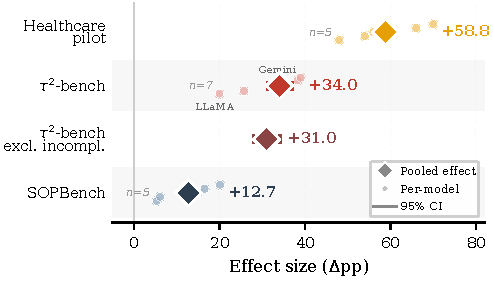
\includegraphics[width=\columnwidth]{figures/fig_cross_benchmark.pdf}
\caption{Cross-benchmark generalization. The ambiguity effect replicates across benchmarks ($n = 19$ model--benchmark data points). Diamonds: pooled effect with 95\% CIs; circles: per-model effects showing cross-model spread (Appendix~\ref{app:sopbench}, \ref{app:healthcare}, \ref{app:model_expansion}).}
\label{fig:cross_benchmark}
\end{figure}

\subsection{Type Partial Ordering (C2)}

\begin{table*}[t]
\centering
\caption{Violation rates (\%) under ambiguous policy clauses by type and model (5.4 = GPT-5.4, 4.1 = GPT-4.1, Cla.\ = Claude, Qw3 = Qwen3, DS = DeepSeek). $\Delta$pp: pooled difference (ambiguous $-$ unambiguous) with Newcombe 95\% CIs. Cluster: TOST equivalence cluster at $\pm 15$\,pp---U = upper bound (separated at all margins), M = mid-tier (6/6 pairwise equivalent), L = lower (separates at $\pm 12$\,pp). Layer grouping (Spec./Ling.) did not survive correction (C3, inconclusive; \S\ref{sec:results}). All per-type $p < 10^{-5}$ (Fisher's exact).}
\label{tab:main_results}
\small
\setlength{\tabcolsep}{4pt}
\begin{tabular}{llrrrrrrr@{\hskip 6pt}cr}
\toprule
Layer & Type & Pooled & 5.4 & 4.1 & Cla. & Qw3 & DS & $\Delta$pp\,[95\% CI] & Cl. & $p$ \\
\midrule
\multirow{3}{*}{\textcolor{speccolor}{Spec.}} & Incompleteness$^\dagger$ & 53.6 & 46 & 58 & 48 & 62 & 54 & +49.2\,[42.2, 55.6] & U & $<\!10^{-37}$ \\
 & Auth.\ Scope$^\ddagger$ & 41.6 & 64 & 46 & 12 & 26 & 60 & +36.0\,[29.1, 42.6] & M & $<\!10^{-22}$ \\
 & Cond.\ Prec. & 36.8 & 34 & 36 & 36 & 40 & 38 & +30.8\,[24.0, 37.4] & M & $<\!10^{-17}$ \\
\midrule
\multirow{3}{*}{\textcolor{lingcolor}{Ling.}} & Lexical & 42.8 & 42 & 34 & 32 & 52 & 54 & +35.2\,[28.0, 42.0] & M & $<\!10^{-20}$ \\
 & Scopal & 39.4 & 42 & 38 & 32 & 37 & 48 & +34.2\,[27.4, 40.7] & M & $<\!10^{-21}$ \\
 & Coreferential & 31.6 & 18 & 32 & 22 & 42 & 44 & +18.7\,[11.5, 25.7] & L & $<\!10^{-6}$ \\
\midrule
\multicolumn{2}{l}{\textbf{Overall}} & \textbf{41.0} & 41 & 41 & 30 & 43 & 50 & \textbf{+34.0}\,[31.3, 36.9] & --- & $<\!10^{-105}$ \\
\bottomrule
\end{tabular}

\vspace{1pt}
{\scriptsize $\dagger$\,Information-addition confound (\S\ref{sec:results}; Appendix~\ref{app:confound}). $\ddagger$\,Lowest cross-judge $\kappa = 0.385$ (dual-judge calibration, $n \approx 17$); $\Delta$token$\,= 36.1$ words, analogous confound. Excl.\ incompleteness: $\Delta = +31.0$\,pp [27.9, 34.1].}
\end{table*}

The six types are not interchangeable. An omnibus $\chi^2$ test on ambiguous-condition violation rates rejects the uniformity null ($\chi^2 = 28.02$, $df = 5$, $p = 3.6 \times 10^{-5}$, Cram\'{e}r's $V = 0.137$). Table~\ref{tab:tost_sensitivity} reveals a margin-dependent equivalence structure: three types achieve equivalence at $\pm 10$\,pp, five at $\pm 12$\,pp, and all six at $\pm 15$\,pp. The resulting partial ordering is exploratory and contingent on the $\pm 15$\,pp SESOI choice (Table~\ref{tab:tost_sensitivity} sensitivity columns show instability below $\pm 12$\,pp). The NMI comparison ($0.23$ vs.\ $0.01$) is threshold-independent.

\begin{table}[t]
\centering
\footnotesize
\caption{TOST equivalence sensitivity across margins. Mid-tier = fraction of the six within-cluster pairs (lexical, auth.\ scope, scopal, cond.\ prec.) that are equivalent. Inc.\ and Cor.\ columns indicate separation from the mid-tier cluster.}
\label{tab:tost_sensitivity}
\begin{tabular}{lcccc}
\toprule
Margin & Equiv.\ pairs & Mid-tier & Inc.\ sep. & Cor.\ sep. \\
\midrule
$\pm 5$ pp & 0/15 & 0/6 & \checkmark & \checkmark \\
$\pm 8$ pp & 0/15 & 0/6 & \checkmark & \checkmark \\
$\pm 10$ pp & 3/15 & 3/6 & \checkmark & \checkmark \\
$\pm 12$ pp & 5/15 & 5/6 & \checkmark & \checkmark \\
$\pm 15$ pp & 8/15 & 6/6 & \checkmark & -- \\
$\pm 18$ pp & 9/15 & 6/6 & \checkmark & -- \\
$\pm 20$ pp & 12/15 & 6/6 & -- & -- \\
\bottomrule
\end{tabular}
\end{table}

Bootstrap clustering ($B = 10{,}000$; Appendix~\ref{app:cluster}) confirms stable extremes across all margins. Cross-model concordance is moderate ($W = 0.398$, $p = 0.072$; Appendix~\ref{app:kendall_w}). Per-type inter-judge agreement ranges from $\kappa = 0.479$ (coreferential) to $0.904$ (lexical; Appendix~\ref{app:per_type_agreement}). For coreferential, whose per-type $\kappa$ falls below the moderate threshold ($n = 34$), random measurement error attenuates effects toward zero, making these estimates conservative. Authorization scope exhibits the widest cross-model spread (Table~\ref{tab:main_results}) and the lowest per-type judge agreement; conclusions about this type carry wider uncertainty than the pooled estimates.

Cross-model judge validation ($\rho = 0.71$--$0.89$; Appendix~\ref{app:cross_judge}) confirms type-ranking stability when model composition is held constant; the low two-group concordance ($\rho = -0.03$; Appendix~\ref{app:judge_group_ranking}) reflects differential vulnerability to authorization scope$^\ddagger$, not ranking instability. The partial ordering has robust extremes (incompleteness as upper bound and coreferential as lower bound, replicated across seven models and three judges) with model-composition-dependent mid-tier structure. Core findings remain robust when excluding authorization scope entirely ($\Delta = +33.6$\,pp; Appendix~\ref{app:sans_auth}).

Incompleteness ranks highest in three of five models ($\geq$46\% in all seven; Appendix~\ref{app:model_expansion}); its 49.2\,pp effect is an upper bound (Appendix~\ref{app:confound}). C3 (layer grouping) did not survive Holm--Bonferroni correction ($p = 0.017$, threshold $0.0125$). \label{sec:c4}C4 (model$\times$type interaction) is driven solely by authorization scope (Appendix~\ref{app:c4_sans_auth}).

